%-----------------------------------------------------------------------
%                          hires2_correction.tex
% A&A LaTeX class (aa.cls)
%-----------------------------------------------------------------------
%\documentclass[referee]{aa}    % for a referee version
\documentclass{aa}
\usepackage{graphicx}
\usepackage{txfonts}
\usepackage{placeins}
\usepackage{natbib}
\usepackage[colorlinks,allcolors=blue,bookmarks=false]{hyperref}
\usepackage{xcolor}
\usepackage{amsmath}
\hyphenation{get-sources get-filaments get-images non-uniform back-ground}

\newcommand{\draftnote}[1]{\textcolor{magenta}{\textbf{[#1]}}}
\newcommand{\chg}[1]{\textcolor{magenta}{#1}}
\newcommand{\mH}{m_{\rm H}}
\newcommand{\muH}{\mu_{\rm H_2}}
\newcommand{{\um}}{\,$\mu$m}
\newcommand{\Teff}{T_{\rm E}}
\newcommand{\Sc}{\mathcal{D}_{\rm c}}
\newcommand{\Sim}{\mathcal{D}}
\newcommand{\Iim}{\mathcal{I}}
\newcommand{\Sig}{\Sigma}
\newcommand{\Ssh}{\Sigma_{\rm s}}
\newcommand{\Sbase}{\Sig_{\rm b}}

\begin{document}

\title{Correcting the temperature bias of dust surface density\\images of molecular clouds}

\author{Alexander Men'shchikov\inst{1}}
\institute{D\'epartement d'Astrophysique (DAp), IRFU, CEA Saclay,
Universit\'e Paris-Saclay, 91191 Gif-sur-Yvette, France}

\date{Received / Accepted}
\offprints{Alexander Men'shchikov}
\titlerunning{Correcting the temperature bias of surface density images}

\abstract{Surface densities of molecular clouds are obtained by fitting a single modified blackbody to the far-infrared intensities
of dust emission in each pixel. A line of sight crossing a dense structure is not isothermal, the fit is weighted toward the warmer
material, and the surface density is underestimated by up to a factor of three. We show first that the deficit cannot be measured
from the observed spectral energy distributions: its signature is 1.0 to 5.8\% of the intensities while the deficit itself is 9 to
38\%, so any scheme that infers one from the other amplifies relative photometric errors by a factor of 7 to 9, beyond the accuracy
of the photometry. The correction must therefore be calibrated externally, and we calibrate it on a grid of radiative transfer
models. A single relation between the dust temperature and the effective column of material shielding it describes 750 shells of 15
models spanning a factor of 256 in the surface density of the embedding cloud, a factor of 12 in core size and a factor of 270 in
central-to-edge density ratio, with a mass-weighted scatter of 3.6\%. The shielding column is obtained by averaging over the
directions from which the radiation arrives, which removes the geometry from the problem: a uniform sphere, a uniform cube and a
plane-parallel layer of the same observed column give corrections within 10\% of one another, and the plane-parallel layer is the
extreme case because it alone is unbounded across the line of sight. The result is the correction factor as an explicit function of
the surface density that an image holds, with no fitted constants. It applies to any surface density image made by fitting one
modified blackbody per pixel, at the resolution of the longest waveband. It also applies at higher resolution, because in the
multi-resolution reconstruction produced by \emph{hires} the whole of the integrated deficit resides in the base image formed at
the coarsest resolution, so that one additive correction of that image corrects every image of the reconstruction. On a simulated
sky containing a diffuse cirrus, filaments and embedded cores the integrated background-subtracted contribution of the injected
cores is recovered to 1\% of its true value, against 54\% uncorrected, and a core mass measured within one Bonnor-Ebert radius to
better than 1\%, against a loss of 43\%. Applied to a field of the Aquila cloud the correction raises the integrated surface
density by a factor of 1.657 and increases the area above $10^{23}$\,cm$^{-2}$ seventeenfold. The correction is insensitive to
noise, uses no colors and therefore inherits the calibration uncertainty of one waveband only, and is applied once.}

\keywords{ISM: clouds -- ISM: structure -- Stars: formation -- Infrared: ISM -- Submillimeter: ISM -- Techniques: image processing}

\maketitle
\nolinenumbers 

% =====================================================================

\section{Introduction}
\label{sec:intro}

Far-infrared and submillimeter surveys of molecular clouds with the \emph{Herschel} Space Observatory \citep{Pilbratt_etal2010}
have produced the images from which most of what is known about the structure of nearby star-forming regions has been derived
\citep[e.g.][]{Andre+2010, Konyves+2015, Andre+2014}. The physical quantity of interest, the surface density of dust and gas, is
not observed directly. It is obtained by fitting an optically thin modified blackbody to the intensities observed in each pixel
\citep{Hildebrand1983}, which yields one dust temperature and one surface density per line of sight.

Such images are the basis for the extraction of dense cores and filaments, and every quantity derived from them, in particular the
core mass function, inherits their accuracy. Their angular resolution is that of the longest waveband used, $36.3{\arcsec}$ at
500{\um}, unless a differential scheme transfers to them the higher resolution of the shorter wavebands
\citep{Palmeirim+2013}. The implementation used here, \emph{hires}, is described in \citet{Menshchikov2021method} and produces
surface density images at the resolution of any of the observed wavebands. The bias discussed below afflicts the conventional
image and the high-resolution one alike, since both rest on the same fit.

The single-temperature assumption is the weak point of the procedure. It is accurate for diffuse material, whose temperature varies
little along the line of sight, and it fails for a cold dense structure embedded in a warmer cloud. The fitted temperature is
weighted by the emission, hence by the warmer material, and the surface density derived from it is too low. The magnitude of the
effect follows from the logarithmic sensitivity of the Planck function,
\begin{equation}
   \frac{\partial \ln \Sig}{\partial \ln T} = -\,\frac{x_\lambda}{1-{\exp\left(-x_\lambda\right)}}\,, \quad
   x_\lambda \equiv \frac{h c}{\lambda k T}\,,
\label{eq:sensitivity}
\end{equation}
which at $T = 10$\,K equals $-8.99$ at 160{\um}, $-5.78$ at 250{\um}, $-4.18$ at 350{\um}, and $-3.05$ at 500{\um}. Overestimating
the dust temperature of a cold core by only 1\,K therefore lowers the surface density derived from the 500{\um} intensity by 30\%,
and the one derived from the 160{\um} intensity by a factor of 2.3. A modest error in the temperature is a large error in the
surface density.

The bias is not a multiplicative constant that could be absorbed into the assumed dust opacity. It grows with the surface density
of the surrounding cloud, because a denser environment produces a larger temperature contrast along the line of sight, and it grows
with the concentration of the structure, because a more centrally condensed core is more strongly shielded. Two structures of the
same true surface density, observed in different environments, are therefore recovered with different values, and their surface
densities are not comparable.

This paper presents a correction of that bias. It is a correction of an image and not of a particular way of making one: what it
needs is the surface density that a single modified blackbody fit returns at the resolution of the longest waveband, and that is
what any such image holds. The multi-resolution reconstruction is then an important special case rather than the subject, and a
useful one, because we show that the whole of the integrated deficit of a reconstruction resides in its coarsest image, so that
correcting that one image corrects the high-resolution images with it.

Section~\ref{sec:where} shows why the deficit cannot be measured from the observed colors, and where in a reconstruction it
resides. Section~\ref{sec:law} derives, from a grid of radiative transfer models, the relation between the dust temperature and
the column that shields the material. Section~\ref{sec:corr} turns that relation into the correction and states what an image must
supply for it to be applied. Section~\ref{sec:sim} validates it on a simulated sky, Sect.~\ref{sec:aquila} applies it to the
Aquila cloud, and Sect.~\ref{sec:limits} states the uncertainties.

Throughout this paper images are denoted by capital calligraphic characters, for instance $\Iim$ and $\Sim$, to distinguish them
from the scalar quantities that appear alongside them. Surface densities are given as the equivalent number of hydrogen molecules
per unit area, in cm$^{-2}$.

% =====================================================================

\section{Where the deficit resides}
\label{sec:where}

Two questions have to be settled before a correction can be constructed. The first is whether the observations themselves contain
the answer, so that the deficit of a line of sight could be read from the shape of its spectral energy distribution. They do not,
and the reason is quantitative rather than a matter of principle. The second concerns a multi-resolution reconstruction, which is
not one image but a sequence of them: if the deficit were distributed over all of them, each would need its own correction and the
resolution at which the factor is evaluated would matter. It is not distributed, and that is what makes the high-resolution
application as simple as the conventional one.

\subsection{Why the observed colors cannot supply the correction}
\label{sec:amplification}

It is natural to attempt to measure the temperature structure directly, by fitting more than one component to the observed
spectral energy distribution of each line of sight. Without noise this works: a free two-temperature fit over 160 to 500{\um}
recovers between 0.96 and 1.00 of the true surface density at the center of the four models, against 0.62 to 0.91 for the
single-temperature fit. With noise it does not. The reason is quantitative and is set out in Table~\ref{tab:signature}.

\begin{table}
\caption{Signature of the temperature mixing in the four-band spectral energy distribution at the center of each model, compared
with the deficit it produces. Columns two to five give the relative residuals, in percent, of the best single-component fit to the
noiseless intensities; column six their root-mean-square; column seven the fraction of the true surface density that the
single-component fit recovers.}
\label{tab:signature}
\centering
\begin{tabular}{lcccccc}
\hline\hline
\noalign{\smallskip}
$\rho_{\rm c}/\rho_{\rm e}$ & 160 & 250 & 350 & 500 & rms & recovered \\
\noalign{\smallskip}
\hline
\noalign{\smallskip}
1.18  & $+0.92$ & $-1.37$ & $-0.44$ & $+0.93$ & 0.97 & 0.914 \\
1.28  & $+0.88$ & $-2.16$ & $-0.46$ & $+1.82$ & 1.50 & 0.869 \\
4.47  & $+3.46$ & $-6.44$ & $-1.56$ & $+5.39$ & 4.61 & 0.680 \\
90.8  & $+3.76$ & $-8.04$ & $-1.64$ & $+7.27$ & 5.79 & 0.619 \\
\noalign{\smallskip}
\hline
\end{tabular}
\end{table}

The residual pattern is the same at every model, positive at 160 and 500{\um} and negative at 250 and 350{\um}, which is the
broadening of the spectral energy distribution by a distribution of temperatures. Dividing the deficit by the root-mean-square of
the residuals gives 8.9, 8.7, 6.9 and 6.6: any scheme that infers the deficit from the band-to-band photometry amplifies
relative photometric errors by a factor of 7 to 9. The calibration uncertainties adopted for \emph{Herschel} observations of
Aquila are 20\% at 70 to 160{\um} and 10\% at 250 to 500{\um} \citep{Konyves+2015}, so at the two weakly concentrated models the
entire signature lies below the photometric accuracy. A test that accepts a second component only where it improves the fit
significantly never fires, at any pixel of any model.

\begin{figure*}
\centering
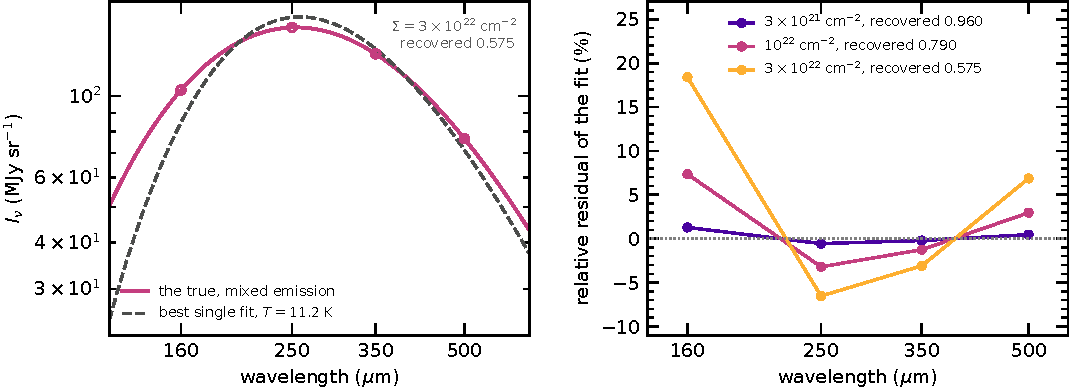
\includegraphics[width=\textwidth]{fig_mixing.pdf}
\caption{\emph{Left}: the emission of a line of sight of $3{\times}10^{22}$\,cm$^{-2}$, the sum over depth of material at every
temperature, with the single modified blackbody fitted to it in the four wavebands and with the weights that the reconstruction
uses. The fit is drawn toward the warmer and brighter material, so the temperature it returns is too high and the surface density
that follows from it is too low. \emph{Right}: the relative residuals of that fit, waveband by waveband, for three total columns,
with the fraction of the true surface density recovered beside each. The pattern is always the same, positive at the ends and
negative in the middle, and it grows with the column, but it never rises above the calibration uncertainties of 20{\%} at
160{\um} and 10{\%} at the three longer wavebands.}
\label{fig:mixing}
\end{figure*}

Figure~\ref{fig:mixing} shows the whole of this in one place: the emission of a mixed line of sight, the single modified
blackbody that is fitted to it, and the residuals that remain. The correction must therefore be calibrated externally, on models
in which the answer is known.

\subsection{The multi-resolution reconstruction}
\label{sec:recon}

Let the observed wavebands be indexed by increasing wavelength $\lambda_i$ with beam half-maximum widths $\theta_i$, and let
$\mathcal{D}(\Iim, T, \lambda)$ denote the optically thin conversion of an intensity into a surface density at the wavelength
$\lambda$ and dust temperature $T$. Writing $G_{\theta_i \rightarrow \theta_{i+1}}$ for the Gaussian kernel that takes the beam
$\theta_i$ to the beam $\theta_{i+1}$, the reconstruction of \emph{hires} builds a base image at the coarsest resolution,
\begin{equation}
\Sim(\theta_N) = \mathcal{D}\!\left(\Iim_N^{\theta_N},\, T_N,\, \lambda_N\right),
\label{eq:base}
\end{equation}
where $T_N$ is the single dust temperature fitted at that resolution, and adds to it one increment per waveband,
\begin{equation}
\Delta_i = \max_{j}\Big[\,\mathcal{D}\!\left(\Iim_i^{\theta_i}, T_j, \lambda_i\right)
        - G_{\theta_i \rightarrow \theta_{i+1}} \ast \mathcal{D}\!\left(\Iim_i^{\theta_i}, T_j, \lambda_i\right)\Big],
\label{eq:increment}
\end{equation}
the maximum being taken over the resolutions at which a temperature is fitted. The image at any resolution is then the cumulative
sum
\begin{equation}
\Sim(\theta_i) = \Sim(\theta_N) + \sum_{i' \ge i} \Delta_{i'}\,.
\label{eq:cumulative}
\end{equation}
Equation~(\ref{eq:cumulative}) has a consequence that determines the design of the correction: an additive correction of the
base image corrects the image at every finer resolution by the same amount, without touching the increments.

\subsection{Decomposition of the deficit by scale}
\label{sec:deficit}

The true surface density decomposes in exactly the same way as Eq.~(\ref{eq:cumulative}), into a term convolved to the coarsest
beam and the differences between successive beams, so the two can be compared term by term. Table~\ref{tab:deficit} does this for
four radiative transfer models of a Bonnor--Ebert sphere embedded in a uniform cloud (Appendix~\ref{sec:grid}), summed over the
source mask at $36.3{\arcsec}$.

\begin{table}
\caption{Ratio of the reconstructed to the true surface density, term by term of Eq.~(\ref{eq:cumulative}), summed over the source
mask at $36.3{\arcsec}$, for four models with central-to-edge density ratios $\rho_{\rm c}/\rho_{\rm e}$. The rows give the base
image at $36.3{\arcsec}$, the sum of the three increments, and the total at $13.5{\arcsec}$. The increments are quoted as a
fraction of the total true surface density, since the true increments nearly cancel and their ratio is meaningless.}
\label{tab:deficit}
\centering
\begin{tabular}{lcccc}
\hline\hline
\noalign{\smallskip}
$\rho_{\rm c}/\rho_{\rm e}$    & 1.18   & 1.28   & 4.47   & 90.8   \\
\noalign{\smallskip}
\hline
\noalign{\smallskip}
base image at $36.3{\arcsec}$  & 0.967  & 0.946  & 0.797  & 0.819  \\
true increments                & 0.000  & 0.000  & 0.000  & 0.000  \\
recovered increments           & 0.021  & 0.025  & 0.026  & 0.006  \\
total at $13.5{\arcsec}$       & 0.988  & 0.970  & 0.824  & 0.825  \\
\noalign{\smallskip}
\hline
\end{tabular}
\end{table}

The true increments carry less than 2\% of the total surface density, because they are unsharp-masking terms whose integral over an
extended region very nearly cancels. The whole integrated deficit therefore resides in the base image. The reconstructed increments
do not cancel, because Eq.~(\ref{eq:increment}) clips them at zero at the shortest wavebands and takes a maximum over
temperatures, and they contribute a spurious positive excess three to six times the true one; that excess happens to act in the
right direction and repairs a few percent of the deficit.

Setting the base image to its true value and leaving the increments untouched would bring the integrated ratios of
Table~\ref{tab:deficit} from 0.988, 0.970, 0.824 and 0.825 to 1.021, 1.025, 1.026 and 1.006. The correction is therefore
formulated for the base image alone, and it acts at the coarsest resolution, where all wavebands share a common beam.

% =====================================================================

\section{What sets the temperature of the dust}
\label{sec:law}

\subsection{The radiation arrives from every direction}
\label{sec:why}

Dust in a molecular cloud is heated by the interstellar radiation field, the ultraviolet and optical light of the stars of the
Galaxy, which arrives from outside the cloud. A grain absorbs that radiation, warms up, and re-radiates in the far infrared, which
is what \emph{Herschel} observed. The temperature a grain settles at is therefore decided by how much radiation actually reaches
it, and that is diminished by the material lying between the grain and the outside.

The radiation arrives from all directions at once, and the material it must cross is different in each of them. Writing $I_0$ for
the unattenuated field, $\kappa$ for the opacity at the wavelengths that do the heating, and $\Sigma_{\rm a}(\hat n)$ for the
column of material the radiation traverses on its way in along the direction $\hat n$, the mean intensity reaching the grain is
\begin{equation}
J = \frac{1}{4\pi}\int I_0\,e^{-\kappa\,\Sigma_{\rm a}(\hat n)}\,{\rm d}\Omega .
\label{eq:meanint}
\end{equation}
We call $\Sigma_{\rm a}(\hat n)$ the attenuating column in the direction $\hat n$. It is a property of the incoming
radiation, not of anything leaving the cloud.

The upper panels of Fig.~\ref{fig:geometry} show what this means for the three shapes a cloud is usually described by. The arrows
are drawn thicker where the radiation has crossed less material, so that the eye sees which directions actually deliver energy.
Deep inside a layer the radiation arrives almost entirely along the normal, because a direction inclined by an angle $i$ has
crossed $1/\cos i$ times as much and grazing directions deliver nothing. At the centre of a sphere every direction has crossed the
same column and none is favoured. Inside a filament the two behaviours are combined: across the filament the path is short, along
its axis it is long, so a filament resembles a sphere in its cross section and a layer along its axis.

Rather than carry an integral over directions into every pixel, we replace the whole angular distribution by the single column
that would produce the same mean intensity. We call it the effective attenuating column $\Sigma_{\rm a}$ and define it by
\begin{equation}
e^{-\kappa\,\Sigma_{\rm a}} \;=\; \left\langle e^{-\kappa\,\Sigma_{\rm a}(\hat n)}\right\rangle_{4\pi} .
\label{eq:seff}
\end{equation}

\begin{figure*}
\centering
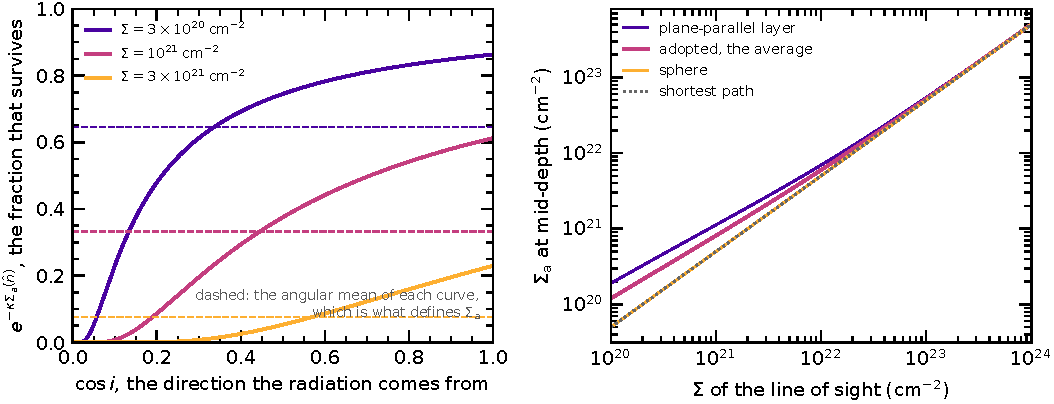
\includegraphics[width=\textwidth]{fig_angular.pdf}
\caption{\emph{Left}: the fraction of the heating radiation that survives the journey inward, against the direction it comes
from, for a parcel at mid-depth of a plane-parallel layer of three total columns. Plotted against the cosine of the angle, the
angular mean of each curve is the area beneath it, drawn dashed; the single column that would produce that same mean intensity is
the effective attenuating column of Eq.~(\ref{eq:seff}). \emph{Right}: that column against the total column of the line of
sight, for the two limiting shapes and for the average of them that is adopted, with the shortest path for comparison.}
\label{fig:angular}
\end{figure*}
It is larger than the column along the shortest path, because the oblique directions contribute less than that path alone would
suggest, and it is the quantity the dust temperature depends on.

Two assumptions are made here and should be stated plainly. The opacity at the heating wavelengths is taken as grey, with
$A_{\rm V} = N({\rm H_2})/0.94\times10^{21}$\,cm$^{-2}$ and $\tau = A_{\rm V}/1.086$; in reality it varies across the ultraviolet
and optical, so Eq.~(\ref{eq:seff}) is an average over wavelength as well as over direction. And the radiation field is taken to
be isotropic outside the cloud, which is what the models of Sect.~\ref{sec:models} assume.

\subsection{The models}
\label{sec:models}

The relation between the effective attenuating column and the dust temperature is not a free choice: it follows from radiative
transfer once the dust and the incident radiation field are fixed. We computed a grid of models with \emph{radmc-3d}
\citep{Dullemond+2012}, each a Bonnor--Ebert sphere \citep{Ebert1955, Bonnor1956} embedded in a uniform cloud and heated from
outside by the interstellar radiation field, which includes the microwave background. The dust opacity is that of
\citet{Ossenkopf+Henning1994}, scaled to the power law $\kappa_\nu = \kappa_0(\nu/\nu_0)^2$ with $\kappa_0 = 9.3057882$\,cm$^2$ per
gram of dust at $\nu_0 = 1000$\,GHz, a dust-to-gas mass ratio of $10^{-2}$ and $\muH = 2.8$. Fifteen nodes are used, spanning a
factor of 256 in the surface density of the embedding cloud, a factor of 12 in the size of the core and a factor of 270 in its
central-to-edge density ratio; they are listed in Appendix~\ref{sec:grid}.

For every shell of every model the density structure is known, so the attenuating column can be computed along any direction by
integrating the density along that ray, and Eq.~(\ref{eq:seff}) evaluated by summing over directions. Shells are weighted by their
mass, so that the innermost cells, where the Monte Carlo temperatures are noisy because few photon packets reach them, carry no
weight.

\subsection{The relation}
\label{sec:relation}

The 750 shells of the 15 models fall on a single relation, which we fit with
\begin{equation}
T(\Sigma_{\rm a}) = T_{\rm f} + (T_0 - T_{\rm f}) \left(1 + \frac{\Sigma_{\rm a}}{\Sigma_\star}\right)^{-\gamma},
\label{eq:law}
\end{equation}
$T_{\rm f} = 6.2090$\,K, $T_0 = 22.4463$\,K, $\Sigma_\star = 2.0738\times10^{21}$\,cm$^{-2}$ and $\gamma = 1.14100$, with a
mass-weighted scatter of 3.6{\%}. The two limits have simple meanings. $T_0$ is the temperature of dust that the radiation
field reaches unimpeded, and $T_{\rm f}$ the temperature it approaches when the radiation cannot reach it at all, the dust then
being warmed only by what little penetrates and by the microwave background, which the models include.

That one relation should describe models so different from one another is the result that makes the method possible, and it is
worth saying why it holds. Neither the size of the core nor its concentration appears in Eq.~(\ref{eq:law}), and neither needs to:
they act on the temperature only by changing how much material lies in the way. The deepest dust temperature of the size series is
3.84, 8.86, 12.71 and 16.96\,K for cores of half-maximum size 0.0214, 0.0572, 0.1196 and 0.2500\,pc, and their maximum attenuating
columns are $2.14\times10^{22}$, $6.72\times10^{21}$, $2.01\times10^{21}$ and $6.26\times10^{20}$\,cm$^{-2}$: the temperature
follows the column and nothing else. The innermost shells of the smallest core reach 3.84\,K, below the floor of the fitted
relation, but they carry a negligible fraction of its mass and the mass-weighted fit is unaffected by them.

% =====================================================================

\section{The correction}
\label{sec:corr}

\begin{figure*}
\centering
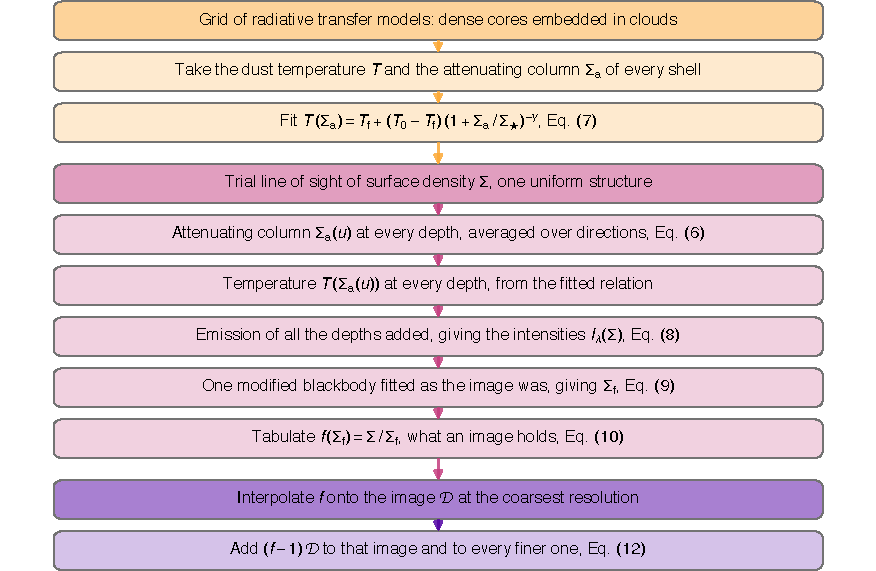
\includegraphics[width=0.75\textwidth]{fig_method.pdf}
\caption{The method step by step. The first group is the calibration, which is done once and yields the temperature relation of
Eq.~(\ref{eq:law}). The second is the calculation of Sect.~\ref{sec:factor}, repeated for every trial surface density, which
yields the table of the correction factor against the surface density that an observed image actually holds. The third is what is
then done to a reconstruction.}
\label{fig:method}
\end{figure*}

\subsection{The calculation}
\label{sec:factor}

Everything needed is now in place, and there is nothing left to adjust. For a line of sight of true surface density $\Sig$:
(\emph{i}) the effective attenuating column of the material at each depth is computed from Eq.~(\ref{eq:seff}), for a structure of
uniform density whose total column is $\Sig$;
(\emph{ii}) its temperature follows from Eq.~(\ref{eq:law});
(\emph{iii}) the emergent intensity is the emission of all the layers added up,
\begin{equation}
   \Iim_\lambda(\Sig) = \kappa_\lambda\,\eta_{\rm dg}\,\muH\,\mH\,\Sig
   \int_0^1 B_\lambda \big(T(\Sigma_{\rm a}(u))\big)\,{\rm d}u ;
\label{eq:emission}
\end{equation}
(\emph{iv}) a single modified blackbody is fitted to it, in the same wavebands and with the same weights that the
reconstruction used, which gives a fitted temperature $\Teff$ and the surface density the reconstruction would report,
\begin{equation}
   \Sig_{\rm f}(\Sig) = \frac{\Iim_{\rm ref}(\Sig)} {\kappa_{\rm ref}\,\eta_{\rm dg}\,\muH\,\mH\,B_{\rm ref}(\Teff)} ;
\label{eq:fitted}
\end{equation}
(\emph{v}) the correction factor is the ratio, tabulated against $\Sig_{\rm f}$ because that, and not $\Sig$, is what an
observed image holds:
\begin{equation}
   f(\Sig_{\rm f}) = {\Sig}/{\Sig_{\rm f}} .
\label{eq:factor}
\end{equation}
Figure~\ref{fig:method} sets out the five steps together with what precedes and follows them.

\begin{figure}
\centering
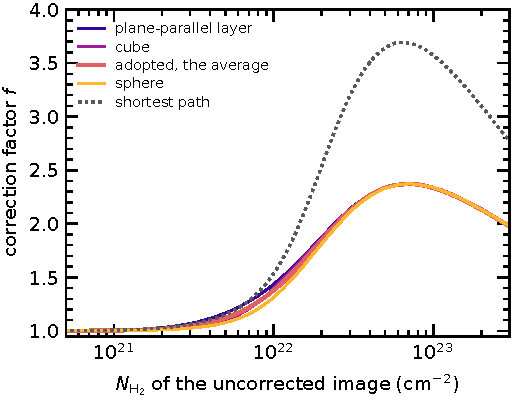
\includegraphics[width=\columnwidth]{fig_relation.pdf}
\caption{The correction factor against the surface density of the uncorrected image, for a uniform plane-parallel layer, for a
uniform sphere, and for the average of the two that is adopted.}
\label{fig:relation}
\end{figure}

Figure~\ref{fig:relation} shows the result. The factor is unity below $10^{21}$\,cm$^{-2}$, where nothing is attenuated, rises
steeply through the range that most of a molecular cloud occupies, and flattens above $10^{23}$\,cm$^{-2}$, where the material is
against the temperature floor and no further shielding can cool it.

The lower panel of Fig.~\ref{fig:geometry} shows the quantity that drives the whole calculation, the run of $\Sigma_{\rm a}$ along
a line of sight. At $10^{21}$\,cm$^{-2}$ it is nearly flat, so the line of sight is nearly isothermal and there is almost nothing
to correct. As the column rises the profile steepens and approaches the dotted line, which is what the shortest path alone would
give: once the material is optically thick the oblique directions deliver nothing and only the normal matters.

\begin{figure*}
\centering
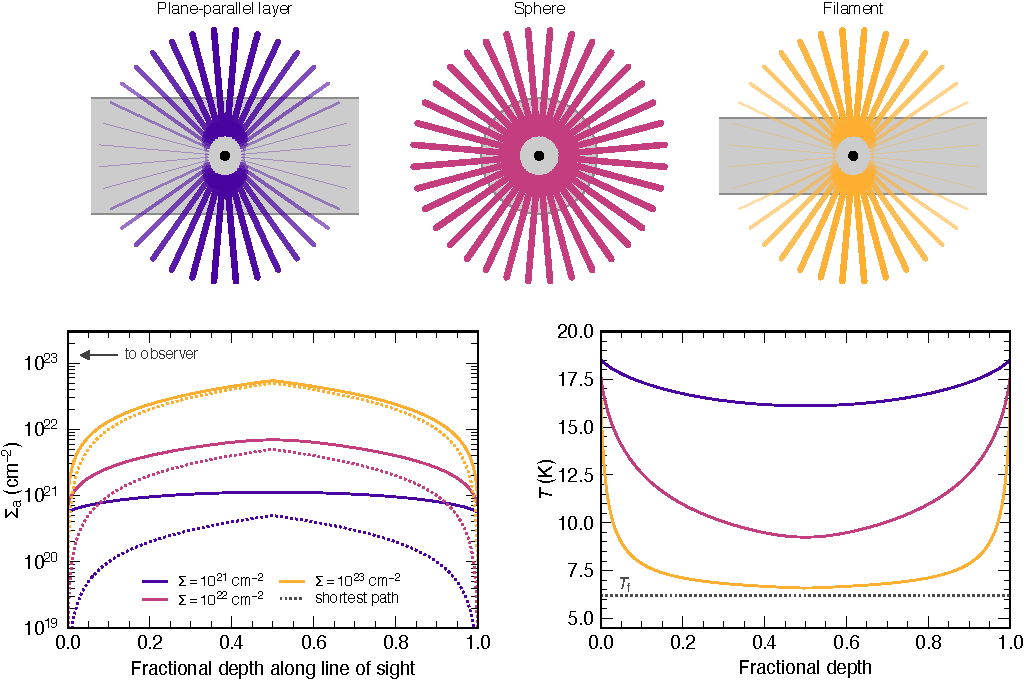
\includegraphics[width=0.8\linewidth]{fig_geometry.pdf}
\caption{\emph{Upper panels}: the radiation that heats a parcel of dust, marked by the black point, arrives from every direction
having crossed columns of very different length. The arrows are drawn thicker where less material has been crossed. In a layer
almost everything arrives along the normal; at the centre of a sphere no direction is favoured; a filament is intermediate, short
across and long along its axis. \emph{Lower panel}: the effective attenuating column of Eq.~(\ref{eq:seff}) along a line of sight
through a layer, as a fraction of the column the observer measures, for three total columns. The dotted line is what the shortest
path alone would give.}
\label{fig:geometry}
\end{figure*}

\subsection{Why the shape hardly matters}
\label{sec:orient}

The calculation needs a shape, and an observed field does not supply one: cores are embedded in filaments, filaments are curved
and blended with their neighbors, and everything sits in a background that fluctuates on every scale. It is therefore important
that the answer should not depend much on which shape is assumed, and it does not.

Figure~\ref{fig:relation} gives the correction computed for a uniform sphere, a uniform cube and a uniform plane-parallel layer
of the same observed column. The three agree to within 10{\%} everywhere, and to 4{\%} or better outside a narrow band
near $10^{22}$\,cm$^{-2}$. The reason
is visible in Fig.~\ref{fig:geometry}: at low column nothing is attenuated and every shape gives unity, while at high column the
deepest material is optically thick in every direction and the distribution of path lengths ceases to matter. Sensitivity to shape
exists only in between, and there the correction itself is modest. Where the geometry would matter, the correction is small;
where the correction is large, the geometry does not matter. We average the sphere and the layer, and take their difference as the
uncertainty the geometry contributes.

The cube is in the figure to show that the two limits are limits. It is a body with none of the symmetry of either, and its
correction falls between them at every column, within 6{\%} of the sphere and 3{\%} of the layer at worst. A layer is
the extreme case and not one shape among several, and the reason is that it is unbounded across the line of sight. For a parcel at
its mid-plane the path to the boundary is the half-thickness divided by the cosine of the angle to the normal, so it diverges as
that angle approaches a right angle and a whole band of directions around the plane of the layer delivers nothing at all, however
thin the layer is made. At $10^{22}$\,cm$^{-2}$ the directions within $30\degr$ of the normal already carry 64{\%} of the
mean intensity and those within $45\degr$ carry 93{\%}. In a bounded body the path is finite in every direction, at most of
the order of the size of the body, and no direction is lost. A sphere is the opposite extreme, since a compact body of a given
central column blocks the least sky that any body of that column can. Every real cloud, of whatever outline, lies between the two,
and the interval between them is the whole of what the shape can contribute. This is why the method needs no statement about the
shape of the cloud it is applied to.

The dotted curve of Fig.~\ref{fig:relation} shows what is lost by ignoring the angular average altogether and using only the
column along the shortest path, with the geometric factor of one quarter that a sphere, a layer and a filament all share once
averaged over their bodies and over isotropic orientations. Below $3{\times}10^{21}$\,cm$^{-2}$ that cruder treatment agrees
with the full
calculation to 1{\%}, but it diverges above $10^{22}$\,cm$^{-2}$ and overestimates the correction by half at
$10^{23}$\,cm$^{-2}$. The shortest path assigns the deep material more shielding than it has, because the oblique directions
still deliver something, and the fit responds to the whole run of temperature and not to its extreme. The angular average is
therefore not a refinement of the shortest path but a different answer, and it is the one that the models support.

One assumption remains, that each structure is of uniform density, and it matters far less than it appears. Along a
plane-parallel line of sight it does not matter at all. What shields a parcel of dust is the column of material lying between it
and the surface, and that column is what it is however the material within it is distributed: piling half of it into a dense
clump changes nothing about how much of it there is. The mass of a line of sight per unit column is constant as well, for any
density profile whatever, because the column is itself the integral of the density. Writing $\Sig(s)$ for the column in front of
a parcel at the depth $s$, the emission of Eq.~(\ref{eq:emission}) integrated along the line of sight is
\begin{equation}
   \int_0^L B_\lambda\big(T(\Sigma_{\rm a}(\Sig(s)))\big)\,\rho(s)\,{\rm d}s
   = \int_0^{\Sig} B_\lambda\big(T(\Sigma_{\rm a}(\Sig'))\big)\,{\rm d}\Sig' ,
\label{eq:invariance}
\end{equation}
and the density has disappeared. Two lines of sight of the same total column emit the same spectrum whether their material is
smooth or clumped, and whether a clump sits at the near face, in the middle or at the far face.
Appendix~\ref{app:arrange} confirms this numerically on density profiles differing by a factor of thirty, which reproduce the
smooth case to two parts in $10^{4}$.

Concentration and arrangement can therefore act only through the one thing that Eq.~(\ref{eq:invariance}) assumes, that the
radiation leaves along the line of sight rather than across it. They do, and by a modest amount. A sphere whose central-to-edge
density ratio is 10 requires a correction 3{\%} larger than a uniform sphere of the same central column, and one whose ratio
is $10^3$ requires between 6 and 15{\%} more, the difference growing with the column. A cirrus with a denser structure
embedded in it requires between 15{\%} less and 11{\%} more than the single uniform body that the method substitutes
for it, according to where within the cirrus the structure lies. Both are measured in Appendix~\ref{app:arrange} and enter the
budget of Sect.~\ref{sec:limits}.

\subsection{How it is applied}
\label{sec:apply}

The correction of an observed field requires the base image alone:
\begin{equation}
\Sc(\theta_i) = \Sim(\theta_i) + \big[f\big(\Sim(\theta_N)\big) - 1\big]\,\Sim(\theta_N) .
\label{eq:correction}
\end{equation}
The amount in brackets is computed once, from the image at the coarsest resolution, and added unchanged to the image at every
resolution, which Eq.~(\ref{eq:cumulative}) permits because the increments do not depend on the base image. Two practical
consequences follow. The correction must be evaluated on the coarsest image and not on a finer one: $f$ rises with surface
density, and a finer image has sharper peaks, so evaluating $f$ there would return a larger and unvalidated factor. And the
correction is not idempotent, so it must be applied once; both of our implementations stamp their output and refuse an input that
has already been corrected.

\subsection{What the correction needs, and what it does not}
\label{sec:needs}

Nothing in Eqs.~(\ref{eq:seff}) to (\ref{eq:factor}) refers to the multi-resolution reconstruction. The factor is a function of
one number, the surface density that a single modified blackbody fitted to the observed intensities returns at the resolution of
the longest waveband, and that number can be obtained from the observed images alone. The base image of \emph{hires} is precisely
that fit and nothing else, which we verified directly on the grid: a single modified blackbody fitted here to the same wavebands
with the same weights reproduces the base image that \emph{hires} writes to better than 1{\%} at every node. The correction
therefore applies to a conventional surface density map made in the usual way from the \emph{Herschel} intensities convolved to a
common beam, whether or not \emph{hires} has been run, and Eq.~(\ref{eq:correction}) then reduces to multiplying that map by
$f$.

What the reconstruction supplies, and what no correction can replace, is the increments: the information on scales finer than the
longest waveband. Without them there is nothing at $13.5{\arcsec}$ to correct, and the corrected map is a map at
$36.3{\arcsec}$. The base image is therefore not an ingredient that has to be provided from outside; it is the anchor to which
the correction is attached, and it can be computed wherever the intensities are. The increments are the part that has to come
from somewhere else.

The order matters when the image is to be decomposed. The shielding of a parcel is set by the whole column along its line of sight,
so the factor has to be evaluated on the total surface density and not on any component of it. Correcting first and separating the
background afterwards recovers the crest of a filament above its background to 2{\%}; separating first and correcting the
background-subtracted structure, which evaluates the factor at a column the material does not have, recovers only 73{\%} of it. For
the same reason the correction must never be applied to an image that already carries it, nor to a true surface density: applying
the factor to the true image of the simulated sky would multiply the crest of a filament by a further 2.16.

One condition attaches to using the correction outside \emph{hires}. The table of $f$ is built for a particular set of wavebands
and a particular weighting of them, because the fitted surface density $\Sig_{\rm f}$ depends on both, and it must be rebuilt if
the map to be corrected was made from a different set or with different weights. It cannot, on the other hand, be replaced by
anything read from the photometry itself, for the reason given in Sect.~\ref{sec:amplification}: the signature of the temperature
mixing lies below the calibration uncertainties, so the correction has to come from the models whatever image it is applied to.

Two further properties follow immediately from the construction. The correction is insensitive to noise, because it evaluates a
smooth function of an image rather than fitting anything: adding Gaussian noise of 1.5, 0.50, 0.30 and
0.15\,MJy\,sr$^{-1}$ at 160, 250, 350 and 500{\um} changes the integrated corrected surface density of the models by less than
0.5\%. And it depends on the
photometric calibration of the reference waveband only, in exact proportion, because the base image is proportional to that one
intensity; the amplification by 8 to 10 found in Sect.~\ref{sec:amplification} does not apply, since the colors are not used.

% =====================================================================

\section{Validation on a simulated sky}
\label{sec:sim}

The models of Sect.~\ref{sec:relation} are single spheres, and an observed field is not. We therefore built a simulated sky
containing a diffuse cirrus, filaments and embedded cores, in which the true surface density is known by construction and every
component obeys Eq.~(\ref{eq:law}) with the geometry it should have: the cirrus plane-parallel, the filaments cylindrical with the
cross-section observed in real clouds, the cores spherical and taken from the same radiative transfer grid. The intensities were
computed at 70 to 500{\um}, convolved to the corresponding beams, sampled on $3{\arcsec}$ pixels and passed through \emph{hires}
exactly as an observation would be.

Figure~\ref{fig:simsky} shows the sky before and after correction beside the truth, and Table~\ref{tab:sim} gives the numbers at
both resolutions. The cores are recovered well: their central pixels to 1{\%} at $13.5{\arcsec}$ and to 7{\%} at $36.3{\arcsec}$,
and the integrated background-subtracted core, which is the quantity a mass is measured from, to better than 1{\%}. Integrated over
the whole field the correction overshoots by 11{\%}, and the reason is the superposition discussed in Appendix~\ref{app:arrange}:
most of the area of the field is diffuse, its cirrus and its filaments shield each other less than the single connected body that
the correction assumes, and the overshoot is of the size that Fig.~\ref{fig:superposition} leads one to expect. A core dominates
its own line of sight and is described well; an extended diffuse region is where the assumption is weakest.

\begin{table}
\caption{Recovered fraction of the true surface density of the simulated sky at both resolutions, for filaments lying in the plane
of the sky and for filaments inclined at random. The values at the cores are medians over the 95 injected cores at their central
pixels, and the last line is the median of the integrated background-subtracted core within one Bonnor-Ebert radius.}
\label{tab:sim}
\centering
\begin{tabular}{lcccc}
\hline\hline
\noalign{\smallskip}
 & \multicolumn{2}{c}{plane of the sky} & \multicolumn{2}{c}{inclined at random} \\
\noalign{\smallskip}
\cline{2-3}\cline{4-5}
\noalign{\smallskip}
 & uncorr & corr & uncorr & corr \\
\noalign{\smallskip}
\hline
\noalign{\smallskip}
$36.3{\arcsec}$ integrated   & 0.774 & 1.104 & 0.786 & 1.131 \\
$13.5{\arcsec}$ integrated   & 0.776 & 1.106 & 0.788 & 1.133 \\
$36.3{\arcsec}$ at the cores & 0.728 & 1.070 & 0.728 & 1.070 \\
$13.5{\arcsec}$ at the cores & 0.535 & 0.999 & 0.542 & 1.002 \\
$13.5{\arcsec}$ bg-sub core  & 0.559 & 1.025 & 0.555 & 1.007 \\
\noalign{\smallskip}
\hline
\end{tabular}
\end{table}

\begin{figure*}
\centering
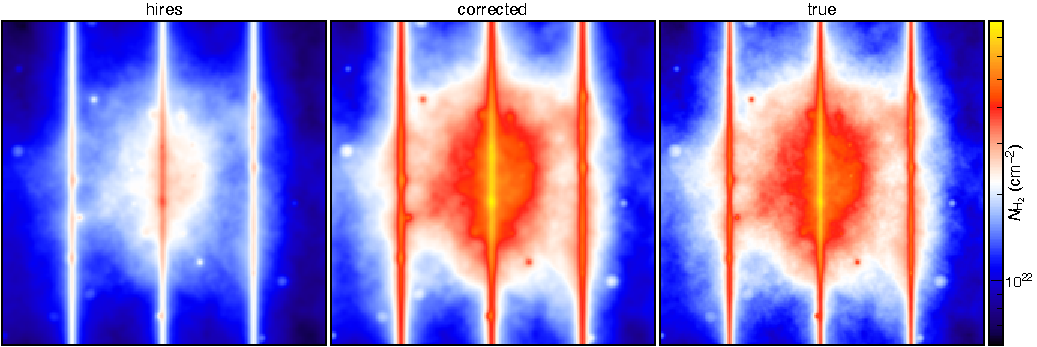
\includegraphics[width=\textwidth]{fig_simsky.pdf}
\caption{A part of the simulated sky at $13.5{\arcsec}$: the reconstruction of \emph{hires}, the same image after the correction
of Eq.~(\ref{eq:correction}), and the true surface density. The three panels share one logarithmic scale.}
\label{fig:simsky}
\end{figure*}

\begin{figure}
\centering
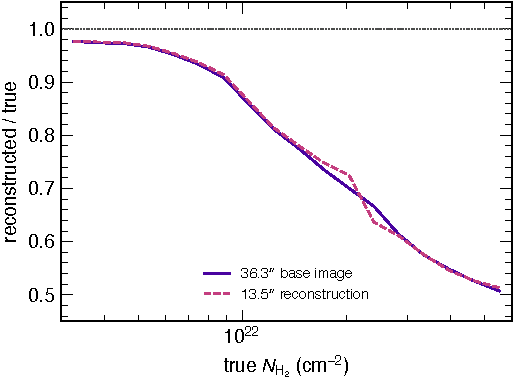
\includegraphics[width=\columnwidth]{fig_deficit.pdf}
\caption{The reconstruction of the simulated sky compared with its true surface density, bin by bin in the true surface density,
at the coarsest resolution and at the finest. The two curves lie almost on top of one another: the increments that the
reconstruction adds between those resolutions are very nearly right, and the whole of the deficit is carried by the base image.}
\label{fig:deficit}
\end{figure}

Figure~\ref{fig:deficit} makes the same point on the simulated sky that Table~\ref{tab:deficit} makes on the models. The
reconstruction falls below the truth by the same fraction at both resolutions at every surface density, so the deficit is
entirely in the base image and a single additive correction of that image is enough.

The quantity of most interest to an observer is not the value of a pixel but the mass of a core, and for that what matters is the
integral of the surface density above the local background over the footprint of the source. Figure~\ref{fig:cores} shows that
integral for each of the injected cores, as a fraction of its true value. Before correction the median is 0.448, that is more than
half of the mass of a core is missing; after correction it is 1.021.

\begin{figure}
\centering
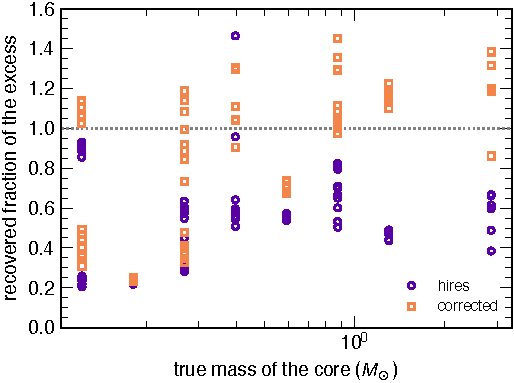
\includegraphics[width=0.85\columnwidth]{fig_core_recovery.pdf}
\caption{Integrated surface density of each injected core above its local background, as a fraction of the true value, before and
after the correction, against the true mass of the core. The dotted line marks a perfect recovery.}
\label{fig:cores}
\end{figure}

% =====================================================================

\subsection{Where the correction fails}
\label{sec:fails}

\begin{figure*}
\centering
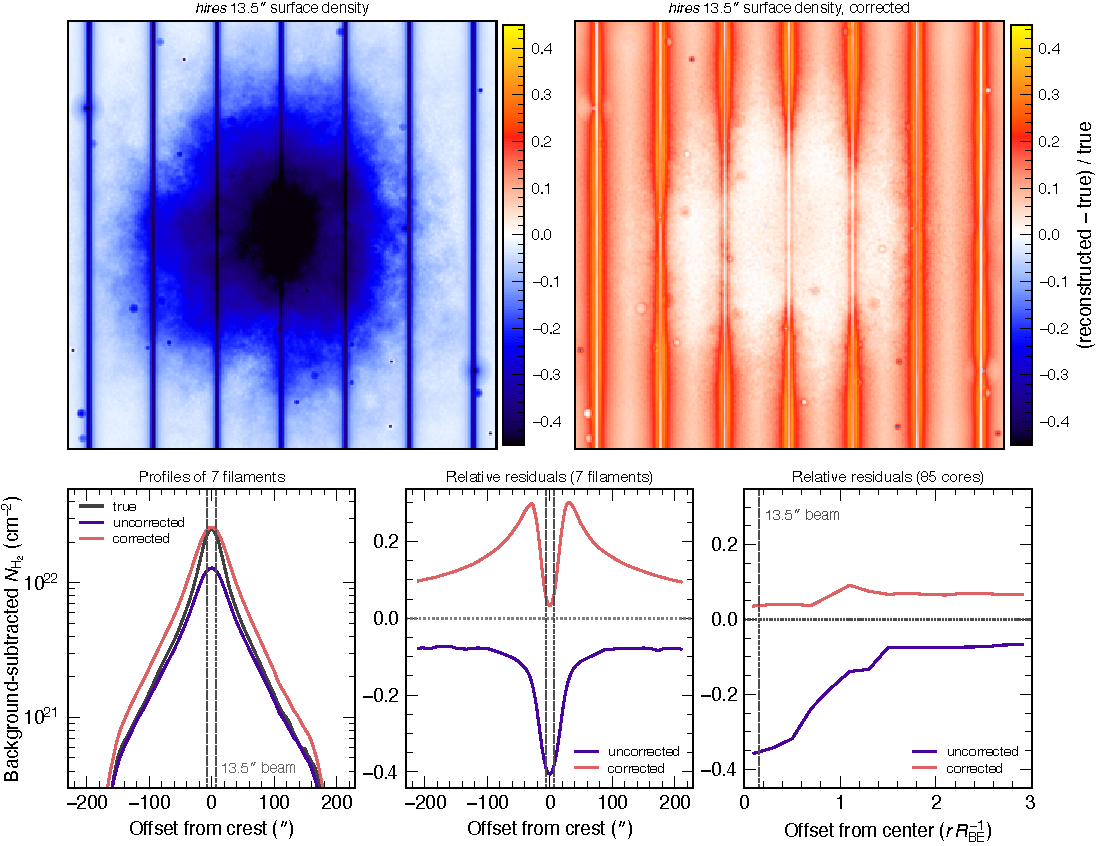
\includegraphics[width=\textwidth]{fig_simsky4_residual.pdf}
\caption{\emph{Upper panels}: the relative residual of the reconstruction at $13.5{\arcsec}$ against the true surface density of
the simulated sky, before and after the correction, on the same scale. \emph{Lower panels}: the profiles themselves, stacked over
the seven filaments and with their backgrounds removed; the same profiles as relative residuals; and the residual stacked over the
injected cores against the radius in units of the Bonnor-Ebert radius. The dashed lines mark the $13.5{\arcsec}$ beam.}
\label{fig:residual}
\end{figure*}

The numbers of Table~\ref{tab:sim} are averages, and it is worth seeing what they average over.
Figure~\ref{fig:residual} shows the residual of the reconstruction against the truth, before and after the correction, as maps and
as profiles stacked over the filaments and over the cores.

Before the correction the reconstruction is too low everywhere: by 8 to 10{\%} over the diffuse field, by 36{\%} at the
centers of the cores and by 40{\%} at the crests of the filaments. After it the diffuse field is recovered to about 10{\%} and
the crests of the filaments to 3{\%}, but a ring of over-correction is left around every compact structure and along
the flanks of every filament. It reaches 30{\%} some $30{\arcsec}$ from a filament crest and 9{\%} at 1.1 Bonnor-Ebert
radii from the center of a core, and it falls away outside.

The ring is not an artifact of the additive form or of the beam. Evaluating the factor on the $13.5{\arcsec}$ image and applying
it there, instead of adding the amount computed at $36.3{\arcsec}$, leaves the flank of a filament exactly where it was, $+0.265$
either way, and makes the crest worse, $+0.095$ against $+0.035$. What produces it is that the factor is a function of the
observed surface density and of nothing else. The shielding of a cylinder falls with impact parameter far faster than the
shielding of a uniform body falls with its column: on the axis a filament is shielded by about half of its axial column, which is
close to what a uniform body of that column would give, so its crest comes out right, while $24{\arcsec}$ away the observed column
is still $2.3{\times}10^{22}$\,cm$^{-2}$ but that material lies near the surface and is barely shielded. A uniform body of
$2.3{\times}10^{22}$\,cm$^{-2}$ would be much colder, so the correction applied there is too large. The rings around the cores are
the same statement for a sphere.

The inclination of a filament acts in the same direction and for the same reason. A filament seen obliquely presents a large
observed column while being shielded only by its radius, so the correction gives it more shielding than it has. Across the seven
filaments of the inclined sky, whose drawn values of $\sin\theta$ are 0.48, 0.76, 0.65, 0.92, 0.91, 0.98 and 0.99, the crests are
over-corrected by 36, 16, 22, 7, 8, 7 and $-1${\%} respectively, in exact order of the inclination.

Nothing in a correction that depends on the observed column alone can remove this, because such a function cannot distinguish
$2{\times}10^{22}$\,cm$^{-2}$ on the flank of a filament from the same column in the body of a uniform structure, and the two need
different corrections. Removing it would require more than one number per pixel, a decomposition of each line of sight into a
smooth component and a structure shielded in its own geometry, which is the calculation of Appendix~\ref{app:arrange} applied
pixel by pixel rather than as an uncertainty. We have not attempted it here.

The shape of a structure is affected as well, and not only its amplitude. Table~\ref{tab:widths} gives the half-maximum widths
and the logarithmic slopes measured on the same profiles.

\begin{table}
\caption{Half-maximum widths of the filaments and of the injected cores, and the logarithmic slope of the filament profiles fitted
between $30{\arcsec}$ and $90{\arcsec}$ from the crest, measured on the true image and on the reconstruction before and after the
correction. The widths are medians over the seven filaments and over the 67 cores measurable in all three images, with the
background taken beyond $180{\arcsec}$ and beyond two Bonnor-Ebert radii respectively. The slope is the index $\alpha$ of a fit of
$A\,r^{-\alpha} + B$ to the unsubtracted profile between $20{\arcsec}$ and $180{\arcsec}$, in which the background level $B$ is
solved for rather than imposed. The filaments of the sky were built with $\alpha = 0.75$.}
\label{tab:widths}
\centering
\begin{tabular}{lccc}
\hline\hline
\noalign{\smallskip}
                              & true & uncorrected & corrected \\
\noalign{\smallskip}
\hline
\noalign{\smallskip}
filament width                & $45.5{\arcsec}$ & $67.1{\arcsec}$ & $65.1{\arcsec}$ \\
core width                    & $64.3{\arcsec}$ & $70.2{\arcsec}$ & $70.5{\arcsec}$ \\
filament slope $-\alpha$      & $-0.82$ & $-0.57$ & $-0.73$ \\
\noalign{\smallskip}
\hline
\end{tabular}
\end{table}

The injected filaments are $40{\arcsec}$ wide and the true image is at $13.5{\arcsec}$ resolution, so $42.2{\arcsec}$ is what a
perfect reconstruction would show; the $45.5{\arcsec}$ measured includes the slope of the cirrus beneath the profile. The
uncorrected reconstruction makes the filaments 47{\%} too wide, and that broadening is not caused by the correction but by
the bias the correction is meant to remove: the crest is suppressed by 40{\%} and the flanks by 21, which flattens the
profile. The correction restores the amplitude, from 0.51 to 1.00 of the true peak, but leaves the width 43{\%} too large,
because the ring of over-correction on the flanks holds the profile open. The cores are much less affected, 9{\%} too wide
before the correction and 10{\%} after.

The slope behaves better than the width, and it is the one shape quantity the correction restores. It has to be measured with the
background as a free parameter, because a constant added to a power law does not leave its logarithmic slope alone: it flattens
it, and removing too much steepens it without limit. The wings of these filaments fall as $r^{-0.75}$, which is so gradual that at
$240{\arcsec}$ the profile still carries a fifth of its value at $30{\arcsec}$, so there is no radius within the spacing of the
filaments at which a background level can be read off safely. Fitting $A\,r^{-\alpha} + B$ to the unsubtracted profile instead,
between $20{\arcsec}$ and $180{\arcsec}$, the true image gives $\alpha = 0.82$ against the $0.75$ with which the filaments were
built, the small excess coming from the beam and from the flattening of the inner profile. The uncorrected reconstruction gives
$0.57$, far too shallow, which is the same statement as the residual profile of Fig.~\ref{fig:residual}: the crest is suppressed
much more than the wings. The correction returns it to $0.73$. So the bias flattens the profile by a third and the correction
removes almost all of that.

There is a choice here that the user of the method should know about. Evaluating the factor on the $13.5{\arcsec}$ image and
applying it there, rather than adding the amount computed at $36.3{\arcsec}$, gives filaments $29${\%} too wide instead of
43 and cores 8{\%} instead of 10, at the cost of the crest, which goes from $+3.5$ to $+9.5${\%}, and of the integrated
recovery, which goes from 1.106 to 1.110. The scheme adopted here therefore favors amplitudes and integrated quantities, which is
what a core mass is measured from, over the widths of extended structures. Anyone measuring the width of a filament from a
corrected image should be aware that the width is not restored by the correction and was not right before it either.

\begin{figure*}
\centering
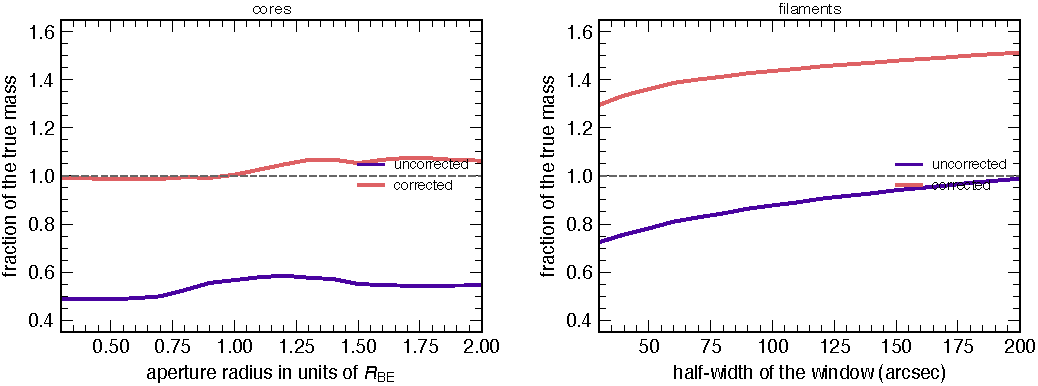
\includegraphics[width=\textwidth]{fig_masses.pdf}
\caption{Masses recovered from the simulated sky, as fractions of the true values, before and after the correction.
\emph{Left}: the mass of a core, against the radius of the aperture, with the background taken between 2 and 2.5 Bonnor-Ebert
radii. \emph{Right}: the mass per unit length of a filament, against the half-width of the window over which the profile is
integrated, with the background level taken from the fit of $A\,r^{-\alpha} + B$ described in the text. Both are medians, over
the injected cores and over the seven filaments.}
\label{fig:masses}
\end{figure*}

The masses are the quantities that matter most, and Fig.~\ref{fig:masses} gives them. They divide sharply. A core mass is
recovered to a few percent: within one Bonnor-Ebert radius the correction returns $1.005$ of the true mass where the uncorrected
reconstruction returns $0.566$, and the inclined sky gives $1.007$ against $0.561$. The curve is flat out to one radius and
drifts upward beyond it, which marks the radius at which the ring begins to enter the aperture. So a core mass function built
from corrected images inherits an accuracy of a few percent, against a factor of nearly two without the correction.

A filament mass per unit length does not fare so well. The ring lies inside any window wide enough to contain a filament, so the
correction overshoots at every window, returning between $1.3$ and $1.5$ of the true value according to how far the profile is
integrated, where the uncorrected reconstruction returns between $0.7$ and $1.0$. An independent estimate of the background,
obtained by
subtracting the image smoothed over $300{\arcsec}$ instead of fitting a level, gives the same picture, $0.750$ uncorrected and
$1.334$ corrected within $\pm120{\arcsec}$. The uncorrected value looks deceptively good because the reconstruction underestimates
the background as well as the filament, and the two errors partly cancel in the difference.

Every curve of Fig.~\ref{fig:masses} is a ratio of the reconstruction to the truth measured by the identical procedure, so an
error of the background that affects the three images alike cancels out of the ratio, and what the filament entries show is the
ring and not the background. The absolute mass of a filament is another matter, and it is uncertain for reasons that have nothing
to do with the correction. Two of them act here. The first is a near-degeneracy: a constant and a tail falling as $r^{-0.75}$ are
almost the same function over any range that can be used, so the fitted level absorbs part of the filament. On these profiles the
fitted $B$ comes out at 0.65 to 0.80 of the true cirrus beneath the crest. The second is the curvature of the background itself.
A background that is convex over the extent of a filament lies above any chord drawn across it, so an interpolated level is too
low; and because that error is largest directly beneath the filament and vanishes at the interpolation points, it adds a centrally
peaked bump to the profile, which inflates the mass and steepens the measured index rather than merely shifting the zero point.
On the simulated cirrus a chord is accurate to better than 1{\%} over baselines up to $\pm600{\arcsec}$ and underestimates
the level by 13{\%} at $\pm900{\arcsec}$, so the effect is negligible for a core and grows with the extent of the structure.
A further difficulty, discussed by \citet{Menshchikov2016}, is that the background beneath a structure is not the smooth
continuation of its surroundings at all: removing the structure leaves an empty volume in its place, so the background that should
be subtracted has the shape of a crater. Detailed accounts of these problems are given in Sect.~3.4.7 of
\citet{Menshchikov2021method} and Sect.~4.4 of \citet{Menshchikov2023}. None of them is addressed by the correction, and none of
them is made worse by it.

A check on the environment supports that reading. The first and the seventh filaments lie near the edges of the field where the
cirrus is weakest and blends least with them; measured there, the index of the true profile is 0.80 and 0.84, close to the 0.75
with which the filaments were built, and the correction returns 0.70 and 0.73. Their masses per unit length within
$\pm100{\arcsec}$ come out at 1.391 and 1.357 of the true value, the same as the 1.408 of a filament at the center of the field
where the cirrus is strongest. The over-correction of a filament mass is therefore a property of the ring and not of the
environment, whereas the uncorrected mass improves from 0.748 at the center to 0.922 and 0.909 at the edges, which is the
background blending and not the method.

Neither column should be used as an absolute measurement: a filament mass per unit length obtained this way is uncertain at the
level of tens of percent whether or not the correction is applied, and improving it requires the background treatment of the
references above together with the per-pixel decomposition discussed here, not a better aperture.

What survives is what is measured. The ring lies outside the aperture in which a core is measured and inside the annulus in which
its background is estimated, so it raises the background a little and very nearly cancels: the central pixels of the cores are
recovered to 0.1 and 0.2{\%} in the two skies and their integrated excess to 2.5 and 0.7{\%}, against 45{\%}
uncorrected. Quantities integrated over an aperture are therefore accurate to a few percent, while an individual pixel on the
flank of a structure can be over-corrected by up to 30{\%} and the crest of a strongly inclined filament by up to 36{\%}.

\subsection{The choice of the base image}
\label{sec:base}

\begin{figure*}
\centering
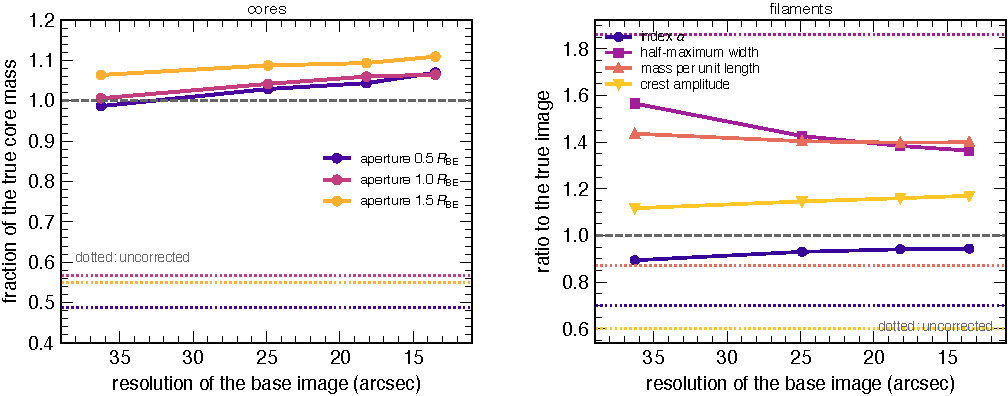
\includegraphics[width=\textwidth]{fig_base.pdf}
\caption{What the choice of the base image costs. The factor is evaluated on the reconstruction at the resolution on the abscissa
and the difference is added to the image at $13.5{\arcsec}$, which is Eq.~(\ref{eq:correction}) with the base taken in turn at
each available resolution. \emph{Left}: the mass of a core recovered within three apertures. \emph{Right}: the shape of a
filament, as ratios to the true image so that one axis serves for all four quantities. Dotted lines mark the uncorrected
reconstruction and dashed lines the true value.}
\label{fig:base}
\end{figure*}

Nothing in Sect.~\ref{sec:corr} ties the correction to the coarsest resolution. The factor is a function of the surface density
that an image holds, and the reconstruction provides an image at each of its resolutions, so any of them may serve as the base.
It is worth knowing what that choice does, and Fig.~\ref{fig:base} measures it.

The behavior is monotonic and the two halves of the figure pull in opposite directions. Taking the base at $36.3{\arcsec}$ gives
a core mass of $1.006$ of the true value within one Bonnor-Ebert radius; moving it to $24.9$, $18.2$ and $13.5{\arcsec}$ gives
$1.042$, $1.060$ and $1.065$. The shape of a filament improves along the same sequence: the index rises from $0.73$ to $0.76$,
$0.77$ and $0.77$ against a true $0.82$, and the half-maximum width falls from $78{\arcsec}$ to $71$, $69$ and $68{\arcsec}$
against a true $50{\arcsec}$. The residual of the field is almost unchanged, from $0.074$ to $0.071$, and the mass per unit
length of a filament is unchanged at $1.40$ to $1.44$, since the ring that sets it does not depend on where the factor is
evaluated.

Two practical conclusions follow. The gain in shape is exhausted by $18.2{\arcsec}$, so there is no continuum of choices worth
tuning: either the coarsest base, or a base one step finer than the middle of the range. And the coarsest base is the one to use
when masses are wanted, which is what a core mass function requires.

We should be explicit about why the coarsest base does so well, because it is not because the correction is exact there. Compared
bin by bin against what the sky actually requires, the factor over-corrects by about 10{\%} per pixel at both resolutions
alike, which is the superposition offset of Sect.~\ref{sec:fails}: the ratio of the required factor to the applied one is $0.88$
to $0.95$ whether it is measured at $36.3{\arcsec}$ or at $13.5{\arcsec}$, agreeing between the two to better than 0.5{\%} in
most bins. The coarse base also under-corrects the peak of a core, because the $36.3{\arcsec}$ beam dilutes it and the
factor rises with the surface density. The two errors have opposite signs and largely cancel, which is where the $1.006$ comes
from. The cancellation is favorable rather than fundamental, and on a field with a different proportion of diffuse and compact
material it would not be exact. It does not affect the recommendation, since the coarse base performs best on both simulated
skies, but the accuracy of a core mass should be quoted as the few percent of Sect.~\ref{sec:limits} and not as the half{\%} of this
test.

This also answers a question that arises naturally: whether the calibration should be redone for a finer base image. It should
not, and it cannot usefully be. The agreement of the two columns above shows that the calibration is a statement about a line of
sight rather than about a beam, and that it transfers unchanged. A calibration built instead from the surface density and the
temperature that the reconstruction itself provides at $13.5{\arcsec}$ would be circular: intensities synthesized from one
temperature and refitted with one modified blackbody return that temperature exactly, and the factor would come out equal to
unity at every column. The physical content of Sect.~\ref{sec:factor} comes from the run of temperature with depth, which a
single reconstructed temperature per pixel does not contain.

% =====================================================================

\section{Application to the Aquila cloud}
\label{sec:aquila}

We applied the correction to a $31\arcmin \times 31\arcmin$ sub-field of the Aquila cloud observed with \emph{Herschel} at 70,
160, 250, 350 and 500{\um} \citep{Andre+2010, Konyves+2015}, adopting a distance of 260\,pc. The reconstruction provides the base
image at $36.3{\arcsec}$ and the image at $13.5{\arcsec}$; the correction is computed from the former and added to both. The
covered area is 375\,769 pixels of $3{\arcsec}$.

The correction factor has a median of 1.363 over the field and a maximum of 2.372, with percentiles at 1, 25, 75 and 99{\%}
of 1.078, 1.249, 1.623 and 2.338. Nowhere in the field is the correction negligible, and nowhere does it exceed the flattening of
Fig.~\ref{fig:relation}. The integrated surface density rises by a factor of 1.657 at $36.3{\arcsec}$ and by 1.649 at
$13.5{\arcsec}$, the two agreeing to 0.5{\%} because the correction is additive and the increments are untouched.

The effect on the distribution of surface density is larger than the median suggests, because the factor rises with the column.
The median of the field moves from $9.7{\times}10^{21}$ to $1.3{\times}10^{22}$\,cm$^{-2}$ and its 99th percentile from
$5.3{\times}10^{22}$ to $1.2{\times}10^{23}$\,cm$^{-2}$. The number of pixels above $10^{22}$\,cm$^{-2}$ grows from 179\,055 to
266\,118, above $3{\times}10^{22}$ from 16\,275 to 64\,483, and above $10^{23}$ from 388 to 6625, a factor of 17. The dense
material of the field is therefore not merely scaled up: a far larger part of the cloud crosses any given threshold once the
temperature mixing is accounted for, which matters directly for any criterion, such as a column threshold for star formation, that
is applied to such an image. The dust temperature implied by the corrected surface densities has a median of 13.18\,K over the
field, with 1 and 99{\%} at 9.29 and 20.47\,K.

The uncertainty to be attached to these numbers is that of Sect.~\ref{sec:limits}, of which the largest terms are the temperature
floor and the arrangement of the material along the line of sight.

\begin{figure*}
\centering
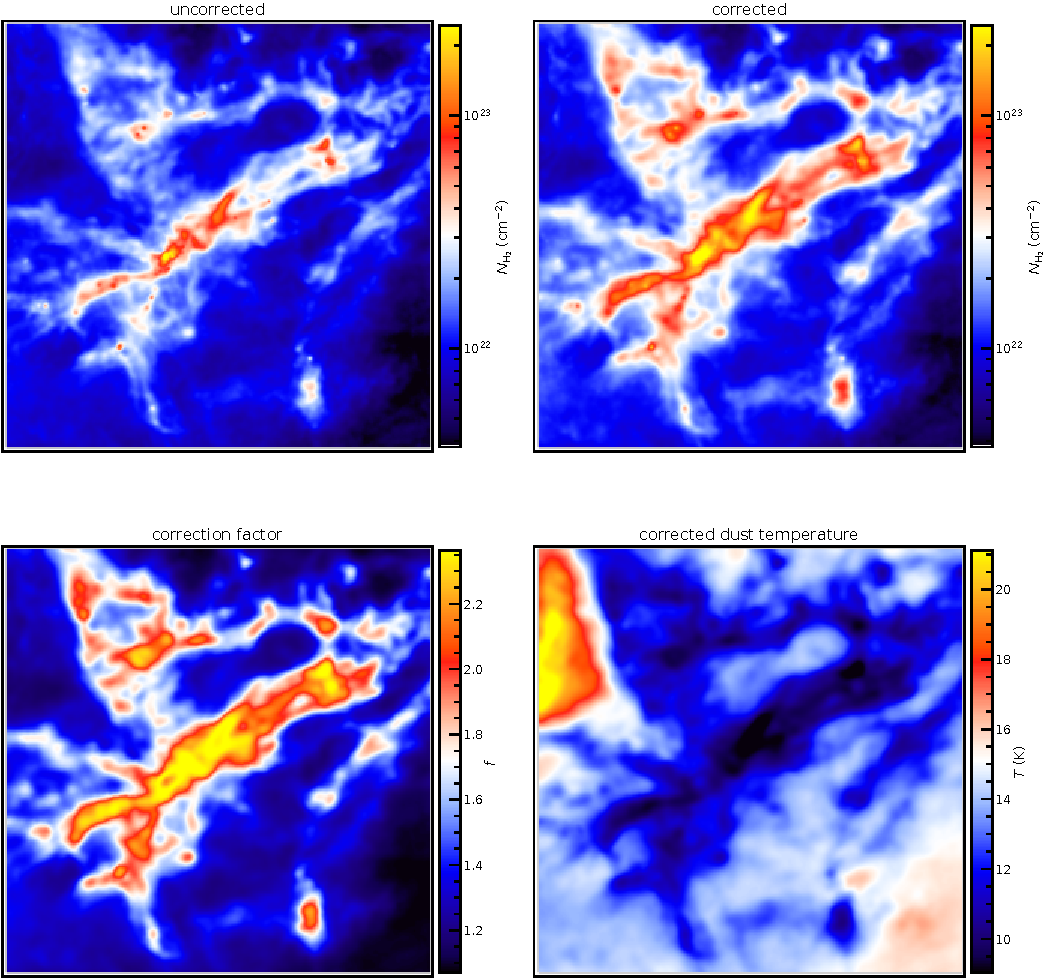
\includegraphics[width=\textwidth]{fig_aquila.pdf}
\caption{The Aquila field at $13.5{\arcsec}$ before and after the correction, on one common logarithmic scale, with the
correction factor interpolated onto the base image and the dust temperature implied by the corrected surface density. The factor
follows the structures: it is least in the diffuse material between them and greatest along the ridges of the filaments and at the
cores, which is where the reconstruction is furthest from the truth and where the masses are measured.}
\label{fig:aquila}
\end{figure*}

Figure~\ref{fig:aquila} shows the field before and after the correction on a common scale, together with the factor and the dust
temperature that follows from the corrected surface density. The factor is not a uniform rescaling: it is smallest in the diffuse
material between the structures and largest along the ridges of the filaments and at the cores, so the contrast of the image
rises as well as its overall level.

% =====================================================================

\section{Uncertainties and limitations}
\label{sec:limits}

\subsection{The shielding relation, and within it the floor}

The magnitude of the correction rests on Eq.~(\ref{eq:law}), and in particular on the temperature that dust approaches when it is
shielded from the interstellar radiation field completely. Our models give 6.4\,K; an analytic relation in common use gives
10\,K; observations of prestellar cores usually place their centers at 7 to 9\,K. Below $10^{22}$\,cm$^{-2}$, which is most of the
area of a typical map, the two relations give corrections that agree to 12 to 20\%, and they diverge above it. The interval
between them should be read as the systematic uncertainty of the method until the floor is settled independently. It is the
largest single uncertainty, and it is a question of physics rather than of method.

\subsection{The geometry}
The calculation needs a shape, and an observed field does not supply one. Figure~\ref{fig:relation} shows that this scarcely
matters:
a uniform sphere and a uniform layer of the same observed column give corrections within 8{\%} of each other everywhere, and
within 4{\%} outside a narrow band near $10^{22}$\,cm$^{-2}$. We average the two and take half their difference as the
uncertainty, which is 5{\%} at worst.

\subsection{The arrangement along the line of sight}

An observed line of sight is not one structure but several, at depths that no observation reveals, and the method replaces them
by a single uniform body of the same total column. Equation~(\ref{eq:invariance}) shows that this substitution is exact in the
plane-parallel limit, so the error it commits is confined to the escape of radiation across the line of sight.
Appendix~\ref{app:arrange} measures it in the two forms it takes. Concentrating a bounded structure raises the required
correction by 3{\%} at a central-to-edge density ratio of 10 and by up to 15{\%} at a ratio of $10^3$. Embedding a
structure in a cirrus changes it by between $-15$ and $+11${\%} according to the depth at which the structure sits, without
a preferred sign, and the value the method applies falls inside that range at every column we examined. We take 15{\%} as
the uncertainty from this source. Section~\ref{sec:fails} shows what it looks like in an image: it is not a uniform offset but
a pattern that follows the structures, small on their crests and largest on their flanks. It is comparable to that of the
shielding relation and larger than that of the geometry, and
unlike either of them it cannot be reduced by a better calculation, because the depth of a structure within a cloud is not an
observable.

\subsection{The peak of a resolved core}

The amount added at a peak is the amount appropriate to the core as the coarsest beam sees it, and a core resolved at the finest
resolution has a somewhat larger deficit than that. Integrated quantities do not suffer from this, and neither does the mass of a
core, which is an integral; only the value of the central pixel of the finest image does.

\subsection{What the correction does not do}

It acts on an image, not on a source. The mass of an individual core additionally requires the subtraction of its background and
the truncation of its footprint, neither of which is addressed here.

It also assumes that the dust is heated from outside, which is what the calibration models are. A line of sight through a
protostar contains an internal source, its temperature gradient is reversed, and Eq.~(\ref{eq:correction}) does not apply. Such
positions should be identified from their compact 70{\um} emission and left uncorrected.

% =====================================================================

\section{Conclusions}
\label{sec:conclusions}

The surface density images of molecular clouds derived by fitting one modified blackbody per pixel are systematically too low
wherever the dust temperature varies along the line of sight, and the deficit reaches a factor of three in the densest material.

The deficit cannot be measured from the observed colors. Its signature in the spectral energy distribution is 1.0 to 5.8\% of the
intensities where the deficit itself is 9 to 38\%, so any method that infers one from the other amplifies relative photometric
errors by a factor of 7 to 9, well beyond the accuracy of \emph{Herschel} photometry. The correction must come from radiative
transfer, and ours does.

What the radiative transfer supplies is a single relation between the dust temperature and the effective column of material
shielding it, which describes 750 shells of models spanning a factor of 256 in the surface density of the embedding cloud, a
factor of 12 in core size and a factor of 270 in central-to-edge density ratio with a mass-weighted scatter of 3.6\%. Size and
concentration enter only through the shielding column. That column is obtained by averaging over the directions from which the
radiation arrives, which leaves nothing to be fitted and nothing to be assumed about the shape of the cloud: a uniform sphere, a
uniform cube and a plane-parallel layer of the same observed column give corrections within 10\% of one another, and the layer is
the extreme case because it alone is unbounded across the line of sight. The relation then gives the correction factor as an
explicit function of the surface density that an image holds, with no fitted constants.

The correction is a correction of an image. It needs only the surface density that a single modified blackbody fit returns at the
resolution of the longest waveband, so it applies to a conventional surface density image of a molecular cloud as it stands. It
applies at higher resolution as well, and this is its most useful application: in a multi-resolution reconstruction the whole of
the integrated deficit resides in the base image formed at the coarsest resolution, because the increments that carry the finer
resolutions are differential terms that very nearly cancel when integrated, so one additive correction of that image corrects
every image of the reconstruction and can be applied after the reconstruction is complete. What such a reconstruction contributes,
and what no correction can replace, is the information on scales finer than the longest waveband.

On a simulated sky containing a cirrus, filaments and embedded cores the integrated background-subtracted contribution of the 
injected cores, which is the quantity a core mass is measured from, is recovered to 1\% of its true value against 54\% uncorrected.
Core masses measured within one Bonnor-Ebert radius are recovered to 0.5{\%}, against a loss of 43{\%} without the
correction, so a core mass function built from corrected images is accurate to a few percent where it was previously wrong by
nearly a factor of two. Masses of extended structures are not so well served: the correction leaves a ring of over-correction on
the flanks of a filament, which lies inside any window wide enough to hold one, and a filament mass per unit length comes out 39
to 53{\%} too high.

Applied to a $31\arcmin{\times}31\arcmin$ field of the Aquila cloud, the correction has a median factor of 1.363 and raises the
integrated surface density by 1.657. The number of pixels above $10^{23}$\,cm$^{-2}$ grows by a factor of 17, so the dense
material of a cloud is not simply scaled but substantially redistributed across any threshold applied to such an image.

The correction is insensitive to noise, it uses no colors and therefore inherits the calibration uncertainty of one waveband only
and in exact proportion, and it has no free parameter at all. Its uncertainties are stated rather than hidden: the temperature
that dust approaches when it is shielded completely, which is a question of physics rather than of method and is the largest of
them; the shape of the structure, which the angular average reduces to 5\%; and the arrangement of the material along the line of
sight, 15\%, which is irreducible because the depth of a structure within a cloud is not an observable.

\begin{acknowledgements}
\draftnote{To be written.}
\end{acknowledgements}

\bibliographystyle{aa}
\bibliography{hires2_correction}

% =====================================================================

\appendix
\nolinenumbers 

\section{The grid of models}
\label{sec:grid}

Table~\ref{tab:grid} lists the nodes. The identifier encodes the three axes of the grid: the index $i$ sets the surface density of
the embedding cloud, $k$ the half-maximum size of the Bonnor--Ebert sphere, and $j$ its central-to-edge density ratio. The three
nodes labeled add\,1 to add\,3 were constructed outside the grid to extend the range of surface density upward. The last column
gives the value of the base image at the central pixel, and is left blank for the four nodes that contribute their tabulated
temperature structure to the shielding relation of Sect.~\ref{sec:relation} but have no synthetic images and therefore do not enter
the tests of Sect.~\ref{sec:sim}.

\begin{table}[ht!]
\caption{Nodes of the model grid used in the calibration. $\Sig_{\rm emb}$ is the surface density of the embedding cloud, $W$ the
half-maximum size of the Bonnor--Ebert sphere, $\rho_{\rm c}/\rho_{\rm e}$ its central-to-edge density ratio, and $\Sbase$ the
value of the base image at the central pixel.}
\label{tab:grid}
\centering
\begin{tabular}{lcccc}
\hline\hline
\noalign{\smallskip}
node & $\Sig_{\rm emb}$ & $W$ & $\rho_{\rm c}/\rho_{\rm e}$ & $\log_{10}\Sbase$ \\
     & (cm$^{-2}$)      & (pc) &                            & (cm$^{-2}$)       \\
\noalign{\smallskip}
\hline
\noalign{\smallskip}
i01j19k13 & $3.75\times10^{20}$ & 0.0572 & 1.18  & 21.21 \\
i01j20k13 & $3.75\times10^{20}$ & 0.0572 & 1.28  & 21.33 \\
i01j22k13 & $3.75\times10^{20}$ & 0.0572 & 1.82  & \ldots       \\
i01j24k13 & $3.75\times10^{20}$ & 0.0572 & 4.47  & 21.77 \\
i01j25k13 & $3.75\times10^{20}$ & 0.0572 & 9.82  & \ldots       \\
i01j26k13 & $3.75\times10^{20}$ & 0.0572 & 27.4  & \ldots       \\
i01j27k13 & $3.75\times10^{20}$ & 0.0572 & 90.8  & 21.89 \\
i01j28k13 & $3.75\times10^{20}$ & 0.0572 & 318   & \ldots       \\
i03j24k13 & $1.50\times10^{21}$ & 0.0572 & 4.72  & 21.82 \\
i05j24k13 & $6.00\times10^{21}$ & 0.0572 & 5.46  & 21.98 \\
i07j24k13 & $2.40\times10^{22}$ & 0.0572 & 7.64  & 21.98 \\
i08j24k13 & $4.80\times10^{22}$ & 0.0572 & 9.48  & 22.44 \\
i09j24k13 & $9.60\times10^{22}$ & 0.0572 & 11.3  & 22.67 \\
i01j24k09 & $3.75\times10^{20}$ & 0.0214 & 83.7  & 21.80 \\
i03j24k09 & $1.50\times10^{21}$ & 0.0214 & 88.5  & 21.86 \\
i05j24k09 & $6.00\times10^{21}$ & 0.0214 & 97.5  & 22.02 \\
i01j24k16 & $3.75\times10^{20}$ & 0.1196 & 1.80  & 21.51 \\
i01j24k19 & $3.75\times10^{20}$ & 0.2500 & 1.32  & 21.08 \\
add\,1    & $1.92\times10^{23}$ & 0.0567 & 1616  & 22.98 \\
add\,2    & $3.84\times10^{23}$ & 0.0525 & 1616  & 23.29 \\
add\,3    & $7.86\times10^{23}$ & 0.0500 & 1616  & 23.80 \\
\noalign{\smallskip}
\hline
\end{tabular}
\tablefoot{The four nodes with a blank last column contribute their tabulated temperature structure to the shielding relation of
Sect.~\ref{sec:relation} but have no synthetic images.}
\end{table}

\section{The arrangement of the material along the line of sight}
\label{app:arrange}

The correction is applied pixel by pixel, and a pixel receives the emission of everything along its line of sight. A single
modified blackbody is fitted to that sum, so what biases the fit is the whole distribution of dust temperatures along the line of
sight and not the temperature of any one structure within it. The method replaces that distribution by the one that a single
uniform body of the same total column would have. This appendix measures what the replacement costs.

\subsection{The invariance}
\label{app:invariance}

For a plane-parallel geometry the emergent emission depends on the total column alone. The attenuating column of a parcel is
determined by the column lying between it and each surface, which does not depend on how that column is distributed, and the mass
of a line of sight per unit column is constant for any density profile, which is Eq.~(\ref{eq:invariance}). As a check on the
algebra and on the integrations, we computed the four intensities of a line of sight of $2{\times}10^{22}$\,cm$^{-2}$ carrying a
clump thirty times the ambient density, placed at 15, 50 and 85{\%} of the depth. They differ from the smooth line of sight
of the same total column by at most $2.1{\times}10^{-4}$, $4.6{\times}10^{-5}$ and $1.2{\times}10^{-4}$, which is the accuracy of
the quadrature. Neither the concentration of the material nor the position of the clump has any effect at all.

\subsection{Concentration}
\label{app:concentr}

Since the density profile leaves the problem entirely in the plane-parallel limit, concentration can act only through the escape
of radiation across the line of sight, which a bounded structure permits and a layer does not. We measure it on a sphere of
density $\rho(r) \propto (1 + r^2/a^2)^{-1}$ out to its boundary, normalized so that the column through its center is the
observed one, with $a$ fixed by the central-to-edge density ratio. The parcels of the central line of sight are weighted by their
density, which is how the emission of that line of sight weights them, and the column that each of them must send its radiation
through is integrated along the ray to the boundary in every direction of the average.

\begin{table}
\caption{Correction factor required by the central line of sight of a sphere of the given central column, for four
central-to-edge density ratios. The first column is the uniform sphere that the method assumes.}
\label{tab:concentr}
\centering
\begin{tabular}{lcccc}
\hline\hline
\noalign{\smallskip}
$\Sig$ (cm$^{-2}$) & uniform & $10$ & $10^2$ & $10^3$ \\
\noalign{\smallskip}
\hline
\noalign{\smallskip}
$5{\times}10^{21}$ & 1.068 & 1.096 & 1.122 & 1.136 \\
$1{\times}10^{22}$ & 1.218 & 1.260 & 1.316 & 1.351 \\
$3{\times}10^{22}$ & 1.709 & 1.750 & 1.857 & 1.968 \\
$1{\times}10^{23}$ & 2.288 & 2.327 & 2.438 & 2.635 \\
\noalign{\smallskip}
\hline
\end{tabular}
\end{table}

Table~\ref{tab:concentr} gives the result. Concentration always raises the required correction, because the mass of a
concentrated structure sits where the shielding is deepest, and the effect grows with the column, from 3{\%} at a ratio of
10 to 15{\%} at a ratio of $10^3$. It is bounded and one-sided, so a correction built on uniform structures underestimates
the deficit of a concentrated one and never the reverse.

\subsection{Two superposed components}
\label{app:twocomp}

The second form of the question is a line of sight crossing a diffuse cirrus with a denser structure embedded in it at an unknown
depth. We take a plane-parallel cirrus of column $\Sig_{\rm c}$, in which the material at the column depth $x$ is shielded by the
angular average of $x/|\mu|$ toward the observer and $(\Sig_{\rm c} - x)/|\mu|$ away from it, and a uniform sphere whose column
through its center is $\Sig_{\rm s}$, embedded in that cirrus with the fraction $q$ of the cirrus column in front of it. A parcel
at the signed position $z$ along the diameter of the sphere, in units of its radius, is shielded by its own sphere over the path
\begin{equation}
   l(z,\psi) = -z\cos\psi + \sqrt{1 - z^2\sin^2\psi} ,
\label{eq:lsphere}
\end{equation}
in units of that radius, and by the cirrus over $q\,\Sig_{\rm c}/|\cos\psi|$ toward the observer and
$(1-q)\,\Sig_{\rm c}/|\cos\psi|$ away from it. The sign of $z$ has to be kept: with $|z|$ in its place the sphere would be
symmetric about its center whatever lay in front of it, and the answer would be wrong for every $q$ but one half. The angular
average of Eq.~(\ref{eq:seff}) is then taken over $\psi$ with the isotropic weight $\sin\psi$, the temperature of every parcel
follows from Eq.~(\ref{eq:law}), the emission of the cirrus and of the sphere are added with their masses, and one modified
blackbody is fitted to the sum exactly as the reconstruction fits it. The correction factor is the ratio of the true column to
the fitted one, as in Eq.~(\ref{eq:factor}). The construction is symmetric under $q \rightarrow 1-q$, as it must be, and the
computed factors are.

\begin{figure*}
\centering
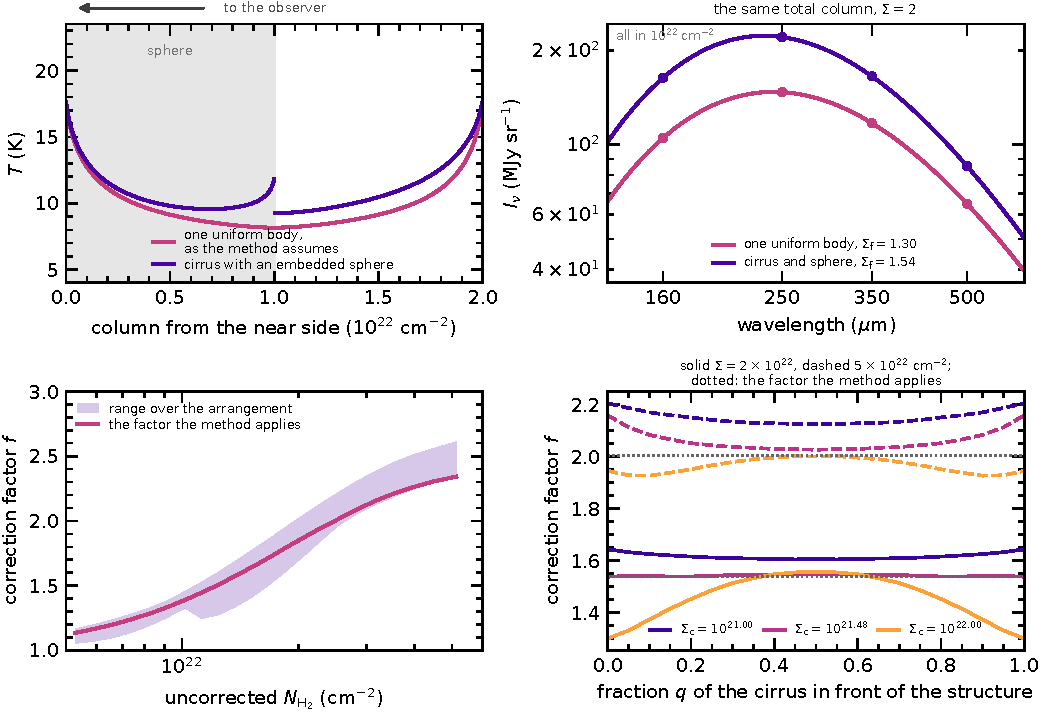
\includegraphics[width=\textwidth]{fig_superposition.pdf}
\caption{\emph{Upper left}: the dust temperature along a line of sight of $2{\times}10^{22}$\,cm$^{-2}$, as the method assumes it
and as it would be if half of that column were a cirrus and half a uniform sphere pressed against its near face. The sphere is
warmer because it loses radiation across the line of sight and has nothing in front of it. \emph{Upper right}: the emission that
follows, with the single modified blackbody fitted to each, and the surface density that each fit returns. The two lines of sight
carry identical columns and nothing observable distinguishes them. \emph{Lower left}: the correction factor, the curve that the
method applies and the range spanned by embedding a sphere in a cirrus of $10^{21}$, $3{\times}10^{21}$ and
$10^{22}$\,cm$^{-2}$ at every position within it. \emph{Lower right}: the same factor against the fraction $q$ of the cirrus
lying in front of the structure, symmetric about $q = 0.5$ as it must be, with the value the method applies dotted.}
\label{fig:superposition}
\end{figure*}

Figure~\ref{fig:superposition} gives the result. The departure from the value that the method applies runs from $-15$ to
$+11${\%}, it has no preferred sign, and the value of the method lies inside the range spanned by the arrangement at every
column.
The spread is largest, 20{\%}, when the diffuse component carries half of the column, and it is below 10{\%} in most of
the configurations examined. The lower right panel shows the dependence on the depth at which the structure sits: it is symmetric
about the mid-plane, as it must be, and weakest when the diffuse component is a small part of the column.

The middle panel of Fig.~\ref{fig:superposition} shows why the effect exists at all, and that it is a property of the fit rather
than of the geometry. The two lines of sight drawn there carry exactly the same total column, but in one of them half of it is a
sphere at the near face of the cirrus, where it loses radiation sideways and has nothing in front of it to block the incoming
field. That arrangement is warmer, it is brighter in all four wavebands, and the single modified blackbody fitted to it returns
$1.54{\times}10^{22}$\,cm$^{-2}$ where the uniform body returns $1.30{\times}10^{22}$\,cm$^{-2}$. The same true column would
then need a correction of 1.30 rather than 1.54.

Nothing observable distinguishes the two. The depth of a structure within a cloud is not a measurable quantity and no improvement
of the calculation can recover it, so the 15{\%} of Sect.~\ref{sec:limits} is an irreducible uncertainty of any method of
this kind rather than a defect of this one.

\end{document}
